%%
%% sample document for AAMAS'18 conference
%%
%% modified from sample-sigconf.tex
%%
%% see ACM instructions acmguide.pdf
%%
%% AAMAS-specific questions? n.yorke-smith@tudelft.nl
%%

\documentclass[sigconf]{aamas}  % do not change this line!

%% your usepackages here, for example:
\usepackage{booktabs}
\usepackage{bcprules}
\typicallabel{ClrInt$_4$}
\usepackage{ASL-ASC-JAIR}

%% do not change the following lines
\setcopyright{ifaamas}  % do not change this line!
\acmDOI{doi}  % do not change this line!
\acmISBN{}  % do not change this line!
\acmConference[AAMAS'18]{Proc.\@ of the 17th International Conference on Autonomous Agents and Multiagent Systems (AAMAS 2018), M.~Dastani, G.~Sukthankar, E.~Andre, S.~Koenig (eds.)}{July 2018}{Stockholm, Sweden}  % do not change this line!
\acmYear{2018}  % do not change this line!
\copyrightyear{2018}  % do not change this line!
\acmPrice{}  % do not change this line!

%% the rest of your preamble here

\newcommand{\code}[1]{\texttt{#1}}

\newcommand{\aser}{\textsf{AgentSpeak(ER)}}
\newcommand{\jason}{\textsf{Jason}}
\newcommand{\AandA}{\textsf{A\&A}}
\newcommand{\aanda}{\textsf{A\&A}}
\newcommand{\moise}{\textsf{MOISE}}
\newcommand{\cartago}{\textsf{CArtAgO}}
\newcommand{\jacamo}{\textsf{JaCaMo}}



%%%%%%%%%%%%%%%%%%%%%%%%%%%%%%%%%%%%%%%%%%%%%%%%%%%%%%%%%%%%%%%%%%%%%
\newcommand{\commenttoby}[3]{\sm{#1}{#2 \textbf{--#3}}}
\newcommand{\ste}[2]{\sm{#1}{#2 \textbf{--Ste}}}
\newcommand{\FORGET}[1]{}
\newcommand{\tba}[1]{\color{blue} TO BE ADDED: #1 \color{black}}
\newcommand{\ale}[1]{\color{blue} [ALE]: #1 \color{black}}
\newcommand{\more}{\color{blue} [...] \color{black}}
\newcommand{\tbc}[1]{\color{red} TO BE CLARIFIED: #1 \color{black}}
% \newcommand{\todo}[1]{\color{red} TODO: #1 \color{black}}
\newcommand{\tbd}[1]{\color{orange} TO BE DISCUSSED: #1 \color{black}}
\newcommand{\FIXME}[1]{{{\bf \color{red}{#1}}}}
%%%%%%%%%%%%%%%%%%%%%%%%%%%%%%%%%%%%%%%%%%%%%%%%%%%%%%%%%%%%%%%%%%%%%%


\sloppy
%%%%%%%%%%%%%%%%%%%%%%%%%%%%%%%%%%%%%%%%%%%%%%%%%%%%%%%%%%%%%%%%%%%%%%%%%%%%%%%%%%%%%%%%%%%%%%%%%%%%%%%%%

\begin{document}

\title{AgentSpeak(ER): An Extension of AgentSpeak(L) improving
  Encapsulation and Reasoning about Goals}

% put your title here!
%\titlenote{Produces the permission block, and copyright information}

% AAMAS: as appropriate, uncomment one subtitle line; check the CFP
%\subtitle{Extended Abstract}
%\subtitle{Industrial Applications Track}
%\subtitle{Socially Interactive Agents Track}
%\subtitle{Blue Sky Ideas Track}
%\subtitle{Robotics Track}
%\subtitle{JAAMAS Track}
%\subtitle{Doctoral Mentoring Program}

%\subtitlenote{The full version of the author's guide is available as \texttt{acmart.pdf} document}


% AAMAS: submissions are anonymous for most tracks
\author{Paper \#329}  % put your paper number here!

%% example of author block for camera ready version of accepted papers: don't use for anonymous submissions
%
%\author{Ben Trovato}
%\authornote{Dr.~Trovato insisted his name be first.}
%\orcid{1234-5678-9012}
%\affiliation{%
%  \institution{Institute for Clarity in Documentation}
%  \streetaddress{P.O. Box 1212}
%  \city{Dublin} 
%  \state{Ohio} 
%  \postcode{43017-6221}
%}
%\email{trovato@corporation.com}
%
%\author{G.K.M. Tobin}
%\authornote{The secretary disavows any knowledge of this author's actions.}
%\affiliation{%
%  \institution{Institute for Clarity in Documentation}
%  \streetaddress{P.O. Box 1212}
%  \city{Dublin} 
%  \state{Ohio} 
%  \postcode{43017-6221}
%}
%\email{webmaster@marysville-ohio.com}
%
%\author{Lars Th{\o}rv{\"a}ld}
%\authornote{This author is the
%  one who did all the really hard work.}
%\affiliation{%
%  \institution{The Th{\o}rv{\"a}ld Group}
%  \streetaddress{1 Th{\o}rv{\"a}ld Circle}
%  \city{Hekla} 
%  \country{Iceland}}
%\email{larst@affiliation.org}
%
%\author{Valerie B\'eranger}
%\affiliation{%
%  \institution{Inria Paris-Rocquencourt}
%  \city{Rocquencourt}
%  \country{France}
%}
%\author{Aparna Patel} 
%\affiliation{%
% \institution{Rajiv Gandhi University}
% \streetaddress{Rono-Hills}
% \city{Doimukh} 
% \state{Arunachal Pradesh}
% \country{India}}
%\author{Huifen Chan}
%\affiliation{%
%  \institution{Tsinghua University}
%  \streetaddress{30 Shuangqing Rd}
%  \city{Haidian Qu} 
%  \state{Beijing Shi}
%  \country{China}
%}
%
%\author{Charles Palmer}
%\affiliation{%
%  \institution{Palmer Research Laboratories}
%  \streetaddress{8600 Datapoint Drive}
%  \city{San Antonio}
%  \state{Texas} 
%  \postcode{78229}}
%\email{cpalmer@prl.com}
%
%\author{John Smith}
%\affiliation{\institution{The Th{\o}rv{\"a}ld Group}}
%\email{jsmith@affiliation.org}
%
%\author{Julius P.~Kumquat}
%\affiliation{\institution{The Kumquat Consortium}}
%\email{jpkumquat@consortium.net}
%
%% The example's default list of authors is too long for headers
%\renewcommand{\shortauthors}{B. Trovato et al.}


\begin{abstract}  
  In this paper, we introduce AgentSpeak(ER), an extension of the
  AgentSpeak(L) language tailored to support encapsulation. The
  AgentSpeak(ER) extention allows for significantly improving the
  style of BDI agent programming along relevant aspects, including
  program modularity and readability, failure handling, and reactive
  as well as goal-based reasoning. The paper introduces the novel
  language, formalises the changes in the usual semantics of
  AgentSpeak, illustrate the features of the language through
  examples, and shows results of experiments evaluating the proposed
  language.
\end{abstract}

\begin{CCSXML}
<ccs2012>
<concept>
<concept_id>10010147.10010178.10010219.10010221</concept_id>
<concept_desc>Computing methodologies~Intelligent agents</concept_desc>
<concept_significance>500</concept_significance>
</concept>
</ccs2012>
\end{CCSXML}

\ccsdesc[500]{Computing methodologies~Intelligent agents}

% AAMAS: the ACM CCS are not needed within AAMAS papers
%%
%% The code below should be generated by the tool at
%% http://dl.acm.org/ccs.cfm
%% Please copy and paste the code instead of the example below. 
%%
%\begin{CCSXML}
%<ccs2012>
% <concept>
%  <concept_id>10010520.10010553.10010562</concept_id>
%  <concept_desc>Computer systems organization~Embedded systems</concept_desc>
%  <concept_significance>500</concept_significance>
% </concept>
% <concept>
%  <concept_id>10010520.10010575.10010755</concept_id>
%  <concept_desc>Computer systems organization~Redundancy</concept_desc>
%  <concept_significance>300</concept_significance>
% </concept>
% <concept>
%  <concept_id>10010520.10010553.10010554</concept_id>
%  <concept_desc>Computer systems organization~Robotics</concept_desc>
%  <concept_significance>100</concept_significance>
% </concept>
% <concept>
%  <concept_id>10003033.10003083.10003095</concept_id>
%  <concept_desc>Networks~Network reliability</concept_desc>
%  <concept_significance>100</concept_significance>
% </concept>
%</ccs2012>  
%\end{CCSXML}
%
%\ccsdesc[500]{Computer systems organization~Embedded systems}
%\ccsdesc[300]{Computer systems organization~Redundancy}
%\ccsdesc{Computer systems organization~Robotics}
%\ccsdesc[100]{Networks~Network reliability}


\keywords{}  % put your semicolon-separated keywords here!

\maketitle


%%%%%%%%%%%%%%%%%%%%%%%%%%%%%%%%%%%%%%%%%%%%%%%%%%%%%%%%%%%%%%%%%%%%%%%%%%%%%%%%%%%%%%%%%%%%%%%%%%%%%%%%%
%% start of main body of paper

\section{Introduction}
\label{sec:intro}


%
% About AgentSpeak(L)
%
{\asl} has been introduced in \cite{Rao96}  with the purpose of defining an expressive, 
abstract language capturing the main aspects of the Belief-Desire-Intention architecture~\cite{Bratman88,Georgeff:1987:RRP:1863766.1863818}, featuring a formally defined semantics and an abstract interpreter.
%
The starting point to define the language were real-world implemented systems, namely the
Procedural Reasoning System (PRS)~\cite{Ingrand:1992:ARR:629535.629890} and the Distributed Multi-Agent Reasoning System (dMARS).
%

%
% Concrete APL
% 
{\asl}  and PRS have become a main reference for implementing concrete Agent Programming Languages 
based on the BDI model: 
%
main examples are Jason~\cite{jason06,bordini:07} and ASTRA~\cite{DBLP:conf/prima/CollierRL15}.
%
Besides Agent Programming Languages,  the {\asl}  model has been
adopted as the main reference to development several BDI agent-based
frameworks and technologies~\cite{BordiniMAPlpa,BordiniMAPlta} as well
as serving as inspiration for theoretical work aiming to formalise
aspects of BDI agents and agent programming
languages~\cite{SardinaThangCAN,LouiseAIL,BordiniMCAPL}.


%
% Contribution
%
Existing Agent Programming Languages extended the language with
constructs and mechanisms making it practical from a programming point
of view~\cite{jason06}.
%
Besides, proposals in literature extended the model is order to make
it effective for specific kinds of systems --- e.g., real-time
systems~\cite{Vikhorev:2011:APP:2030470.2030529}, XXX --- or to
improve the structure of programs, e.g. in terms of
modularity~\cite{Madden2010,Nunes2014}.
%%RHB: Not sure what should go in XXX above?

%
Along this line, in this paper we describe a novel extension of the
{\asl} model --- called {\aser} --- featuring \emph{plan
  encapsulation}, i.e. the possibility to define plans that fully
encapsulate the strategy to achieve the corresponding goals,
integrating both the pro-active and the reactive behaviour.
%
% Key points
%
This extension turns out to bring a number of important benefits to
agent programming based on the BDI model, namely:
%
\begin{itemize}
\item improving the overall readability of the agent source code, reducing fragmentation and increasing modularity;
\item enforcing a more goal-oriented programming style, enforcing  yet preserving the possibility to specify pure reactive behaviours, properly encapsulated into plans ;
\item improving intention management, enforcing a one-to-one relation between intentions and goals---so every intention is related to a goal; 
\item improving failure handling, in particular making it easier the management of failures related to plans reacting to environment events;
\end{itemize}
%
% \noindent Besides the benefits in terms of agent programming, the approach reduces the gap between the design level and the programming level,  ...
% \item facilitate goal-based reasoning -- ...
% \end{itemize}

\noindent The remainder of the paper is organised as follows:
%
first we describe in details the motivations that lead to the proposal (Section \ref{sec:motivation});
%
then, we introduce and discuss {\aser},  introducing the main
concepts, syntax and semantics --- first informally  (Section
\ref{sec:proposal}) and then providing the formalisation of some key
aspect (Section \ref{sec:formalisation}).
%
We discuss then the results of a first evaluation that has been
carried out, based on a prototype implementation extending the ASTRA
platform (Section \ref{sec:evaluation}).
%
We conclude the paper discussing related works (Section \ref{sec:related})
and sketching future work (Section \ref{sec:conclusion}).



\section{Motivation}
\label{sec:motivation}

The main motivation behind {\aser} comes from the experience using
agent programming languages based on the {\asl} model, {\jason} and
ASTRA in particular.
%
Yet, these issues are relevant for any language based on the BDI
architecture.
%
The first issue is about the plan model.

% \subsection{Plan encapsulation}
%
In the BDI model, plans are meant to specify the means by which an
agent should satisfy an end~\cite{Rao96}.
%
In {\asl} a plan consists of a rule of the kind \textsf{e : c <- b}.
%
The head of a plan consists of a triggering event \textsf{e} and a
context \textsf{c}.
%
The triggering event specifies why the plan was triggered, i.e., the
addition or deletion of a belief or goal.
%
The context specifies those beliefs that should hold in the agent's
set of base beliefs if the plan is to be triggered.
%
The body of a plan is a sequence of actions or (sub-)goals.
%

%
% THE PROBLEM
%
So in this approach --- as well as in planning, in general --- the
\emph{means} to achieve a goal --- i.e., the body --- is meant to be
fully specified in terms of the actions the agent should execute and
the (sub-)goals the agent should achieve or test.
%
In the programming practice, however, it is often the case that the
strategy (the means) adopted to achieve some goal (the end) would
naturally include also \emph{reactions}, i.e., reacting to events
asynchronously perceived from the environment, including changes about
the beliefs.
% 
That is, an agent is not reacting only to unexpected events so as to
change/adapt its course of actions, but reactivity could be an
effective ingredient of the strategy, of the plan adopted to achieve
some goal.
%
Besides the programming practice, this is often the case if we
consider human activities too. Reactivity is a key ingredient of many
activities that we perform to achieve specific goals, not only to
handle events that represents errors or unexpected situations (for the
current courses of actions).
%
It follows naturally that this is also an opportunity to extend the
plan model so as to fully \emph{encapsulate} also reactions that are
part of the strategy to achieve the goal, as well as the subgoals that
are specific to that particular goal.


%
%
%
In the following, let's refer to plans triggered by event goals
% \texttt{+!g <- ...} 
as \emph{g-plans}, and plans triggered by the
belief change (including percepts) as \emph{e-plans}.
%
The BDI reasoning cycle automatically updates beliefs from percepts,
and this allows us to write down structured plans with courses of
actions that change according to the environment, by exploiting
goals/subgoals and contexts.
%
For instance, as a very simple example, yet capturing the point, let
us consider the goal of printing down all the numbers between N and 1,
stopping if/when a 'stop' percept is perceived.
%
This task can be effectively tackled using only g-plans:

\begin{small}
\begin{verbatim}
+!print_nums(0).
+!print_nums(_) : stop.
+!print_nums(N) : not stop <- println(N); !print_nums(N-1).
\end{verbatim}
\end{small}
%% RHB: should we replace println with .print ??
	
\noindent This is a clean solution, exploiting the context in plans
and the fact that in the reasoning cycle beliefs are automatically
updated given new percepts.
%
More generally, in the {\asl} model the suggested approach to realise
structured activities whose flow can be environment dependent is by
means of (sub-)goals and corresponding plans with a proper context.

In some cases however this approach is not fully effective, and
\emph{e-plans} are needed,
%
in particular every time we need to react \emph{while executing the
  body of a plan}.
%
A typical case occurs when we have actions (or subgoals) in a plan
that could take a long time to complete.
%
For instance, suppose that instead of simply printing we have a
long-term \texttt{elab} goal (it could be even an action):

\begin{small}
\begin{verbatim}
+!elab_nums(0).
+!elab_nums(N) : stop. 
+!elab_nums(N) : not stop <- !elab(N); !elab_nums(N-1).
\end{verbatim}
\end{small}

\noindent Suppose that, realistically, we cannot spread/pollute plans
about the goal \texttt{!elab} with a stop-dependent behaviour.
%
To solve this problem, using the {\asl} model and in BDI architectures
an e-plan can be introduced, using e.g. internal actions to act on the
current ongoing intention:

\begin{small}
\begin{verbatim}
+!elab_nums(0).
+!elab_nums(N) <- !elab(N); !print_nums(N-1).		
+stop <- .abort(elab_nums(_)).
\end{verbatim}
\end{small}
%% RHB: should we change .abort to .drop_intention ?

\noindent The problem here is that the e-plan \texttt{+stop <- ... } is
part of the strategy to achieve the goal \texttt{!elab\_nums}, however
it is encoded as a separate unrelated plan.

% \subsection{Explicit and Implicit Goals}

The use of e-plans to achieve goals is actually an important
conceptual brick of the {\asl} model.
%
Let us consider the robot cleaning example used to describe plans in
{\cite{Rao96}}.
%
One of the plans is:

\begin{small}
\begin{verbatim}
+location(waste,X):location(robot,X) & location(bin,Y)
  <- pick(waste); !location(robot,Y); drop(waste).
\end{verbatim}
\end{small}

\noindent That is, as soon as the robot perceives that there is a
waste in its location, then it can pick it up and bring it to the bin.
%
This plan an essential brick of the overall strategy to achieve the
goal of cleaning the environment --- or to maintain the environment
clean, in a \emph{maintenance goal} view.
%
However, the fact that this plan is useful to achieve that goal is not
explicit in the source code, it remains in the mind of the
programmer/designer.
%
%
%For instance, let's consider the classic toy example about the robot cleaning the environments from something (bombs, waste)~\cite{jason06}:
%
%\begin{small}
%\begin{verbatim}
%@p1
%+bomb(Terminal, Gate, BombType) : 
%  skill(BombType)
%  <- !go(Terminal, Gate);
%      disarm(BombType).
%@p2
%+bomb(Terminal, Gate, BombType) : 
%  ?skill(BombType)
%  <- !moveSafeArea(Terminal, Gate, BombType).
%@p3
%+bomb(Terminal, Gate, BombType) : 
%  not skill(BombType) & not ?skill(BombType)
%  <- .broadcast(tell, alter).
%...
%\end{verbatim}
%\end{small}
%
%This works very well, however it is not fully satisfactory from a conceptual point of view. 
%
The agent reacts to a waste in a location because it has an implicit
goal, which is about cleaning the environment.
%
However, since there are no g-plans about it, there is no explicit
trace in the agent mental structures about this goal.

This problem can also be illustrated with the following
scenario. Consider an agent that includes a set of plans (a module
written by a third party) to handle social obligations. The module has
several e-plans for the different types of obligations:
\begin{small}
\begin{verbatim}
+obligation(Ag,committed(Goal)) : .my_name(Ag)      <- ...
+obligation(Ag,achieve(Goal))   : .my_name(Ag)      <- ...
-obligation(Ag,Goal) : .my_name(Ag) & .intend(Goal) <- ...
...
\end{verbatim}
\end{small}
If for some reason during its execution an agent decides not to follow
these plans anymore (e.g.\ it chooses to become disobedient), it is
difficult to ``disable'' the behaviour of the above plans. Either
these plans have to be changed to consider a particular state of the
agent or the agent removes all these plans from its plan
library. Neither option is simple to
program. % suitable: the third party code could be not modified; we do not have references for these plans to remove them.
Although we can solve the problem, the lack of an explicit goal
stating that the agent intends to be obedient is the cause of this
problem.

%It is worth remarking that it is possible to bypass the problem in concrete languages (e.g. {\jason}), by exploiting specific features/tricks. 
%%
%However the solution is typically far from being satisfactory from a conceptual point of view.
%%
%For instance, about the bombing example - we can introduce an explicit  goal \texttt{!clean\_env} and a plan in which the course of action is simply waiting to perceive the environment is cleaned:
%
%\begin{verbatim}
%+!clean\_env <- .wait(all_bombs_dismantled).
%+bomb(Terminal, Gate, BombType) : skill(BombType)  <- ?
%\end{verbatim}
%
%\noindent On the one hand, this makes it possible to have an explicit intention at runtime about the dismantling bomb activity. However the plan p0 is completely unrelated in the code from the other reactive plans. Besides, when +bomb is perceived, a separate intention wrt the one about the dismantling goal is created. So they are treated as separate, not related activities.

% \subsection{Failure Handling}

This issue impacts also on plan failures handling, which is a very
important aspect of agent programming.
%
In the Jason dialect of {\asl}, we can define plans that handle the
failure of the execution of g-plans (generating the event
\texttt{-!g}), but not of e-plans.
%
So, for example, if there is a problem in the println action in:

\begin{small}
\begin{verbatim}
+stop <- println("stopped").
\end{verbatim}
\end{small}

\noindent the plan execution fails, without any possibility to react
and handle the failure.
%
In order to handle this, a programmer is forced to structure every
e-plan with failure handling using a subgoal:

\begin{small}
\begin{verbatim}
+stop <- !manage_stop.
+!manage_stop <- println("stopped").
-!manage_stop <- println("failure").
\end{verbatim}
\end{small}

\noindent This contributes to making the program longer and verbose,
besides increasing the number of plans to be managed by the
interpreter.

%Besides failure, meta-level actions to manage intentions (plans in execution) at runtime
%works only with g-plans, since they need to specify as argument the specific goal which generated the intention.

\bigskip

To summarise, this is the set of key issues identified for the basic
plan model in the practice of agent programming:
%
\begin{description}
%
\item[Lack of encapsulation:] The strategy to achieve a goal is
  fragmented among multiple plans, not explicitly related to each
  other.
%
\item[Implicit vs. Explicit goals:] Some parts of an agent program may
  have plans for which the goal is implicit.
%
\item[Difficult failure handling:] Failures/errors generated in the
  body of e-plan cannot be directly captured.
%
\end{description}
%%RHB: Are we not talking about the goal-condition and the fact that
%%external events can trigger various plan, one for each intention??



%\noindent This has an impact also on the performance of the agent
%interpreter at runtime. In the traditional model, each reaction
%represented by an e-plan necessarily generates a new intention to
%manage it, increasing the number of plans in execution to be managed
%by the agent reasoning cycle.
%
%This could have also a negative impact on intention selection at
% each reasoning cycle~\cite{DBLP:conf/atal/LoganTY17}.

%\item[Difficult runtime management] -- Intentions generated by e-plans cannot be managed. Besides, as a consequence of point (1), it is not possible to manage (suspend, abort) the intentions related to some goals as a whole.
%
%\item[Runtime overhead] Each reaction (e-plans) is   new intention => new stack. 


\noindent Besides the pure programming level, it is worth noting that
these issues can affect the %whose
software engineering process for agent development.
%%
In particular, at the design level, it is natural to specify
coarse-grained plans fully encapsulating the strategy to achieve or
maintain goals.
%
It would be important then to keep as much as possible the same level
of abstraction when going from the design to programming, and at
runtime too, to support agent reasoning.


%
%\begin{itemize}
%%
%\item Design / Engineering Drawbacks -- weak encapsulation => impact on modularity => impact on many aspects
%
%%
%\item Reasoning drawbacks -- proliferation of intentions => impact on the reasoning cycle, on intention selection
%%
%\end{itemize}



\section{The {\aser} Proposal}
\label{sec:proposal}

To overcome the problems discussed above, we consider two key changes in the plan model. 

%
% 
%
The first one is to extend the plans beyond the simple sequence of actions and goals, so as to include also the possibility to specify a reactive behaviour encapsulated in the plan.
%
Coherently with the {\asl} model, such a behaviour can be expressed in terms of e-plans.
%
% JH: I changed a bit the terminology
Accordingly, a plan becomes the \emph{scope} of ($i$) a sequence of actions (referred as \emph{body actions}), ($ii$) a set of \emph{e-plans}, specifying a reactive behaviour which is active at runtime only when the plan is in execution, and ($iii$) a set of \emph{g-plans}, specifying plans to achieve subgoals that are relevant only in the scope of this plan. The e-plans and g-plans are referred as \emph{sub-plans}.
%
The sub-plans may include also reactions to failures occurring when executing the plan.

%
%
%
The second one is enforcing that e-plans -- as pieces of reactive behaviours -- must always be defined in the context of a g-plan. We are thus  enforcing the principle that an agent does (and reacts) always because of a goal to achieve or maintain.
%
This ensures that programmers explicitly specify what is the goal to achieve even when defining a pure reactive behaviour. 
%
In so doing, at runtime every intention \footnote{As in \asl, an intention is the result of the deliberation to commit to some desire. Briefly, if the agent has an applicable plan for a goal event (i.e.\ a desire), it commits to it by creating an intention based on that plan and starts executing that plan.} has an associated goal being pursued.

In the remainder of the section we first describe in detail the syntax and informal semantics of the new plan model, including simple examples, and then we discuss the key benefits. 

\subsection{Informal Syntax and Semantics}

At the top level, an {\aser} program is a collection of g-plans, whose syntax is exemplified in the following:
%
% CURRENT VERSION 0.2 (in the doc)
%
{\small
\begin{verbatim}
/*  g-plans to achieve goal g in context c */
+!g : c <: gc { 

  <- a; b; ?g1; !g1; !!g2. // body (optional).

  /* e-plans */
  +e1 : c1 <- b1.	
  +e2 : c2 <- b2.
  +!k : true <: b(10) {
    <- a,b,c.
    +e3 : c3 <- b3. // possible old-style plans
  }	
  
  /* e-plans catching failures */
  -!g[error(ia_failed)] : ...
    <- ... catches from failures 

  /* further g-plans */
  +!g1 : c1 <: gc1 { ... }
}
\end{verbatim}}

Like in {\asl}, a g-plan is defined with a head and a body.
%
% JH: avoid to use the term intention here... goal oriented programming. explain intention in the semantics
Besides the triggering event and the context, the head has a third new element: a \emph{goal condition}, optionally written after \texttt{<:}, with the same syntax as the context. While the context is a pre-condition to select a plan as applicable for an event, the goal condition is a post-condition that defines when the goal can be considered as achieved. Any goal created based on this g-plan is considered achieved if and only if this condition holds. If no goal condition is specified, the goal is considered achieved as soon as the body execution completes, as usual in \asl. However, if a goal condition is defined, to finish the body execution is not sufficient to achieve the goal. Notice that if the goal condition becomes true while the body actions are being executed, the execution stopped.

In {\aser} the body is enclosed by \texttt{\{} and \texttt{\}} and is composed of the body actions (after \texttt{<-}) and sub-plans. 
%
Like in {\asl}, as soon as a g-plan is instantiated, the body actions start to execute. The body actions can be empty -- this is the case of g-plans expressing a pure reactive behaviour.
%
The sub-plans of the g-plan are considered as relevant only for events produced by the g-plan execution. Since, they are in the scope of g-plan. 

% GoalCondition is analogous to the context: however, if context can be considered to be as the pre-condition to execute the plan, the GoalCondition are like a post-condition, which corresponds to a declarative description of the goal to be achieved. 
%
%Alternatively, the execution of a plan can be forced to complete by using an internal action .done - this is useful everytime the goal condition cannot be effectively or naturally described as a boolean expression.
%
%If [GoalCondition] is not specified, by default the condition is that all actions of the main sequence have been executed and completed, in continuity with the AS model. This condition is explicitly represented by the new predefined predicate \texttt{.is\_done}.
%
% The body of the plan provides a lexical and runtime scope of the sub-plans, that is:  variables used in the g/c expression are visible also to subplans the lifetime/availability of the sub-plans is limited to the time in which the g-plan is in execution


While a g-plan is executing, it can be \emph{interrupted} by events relevant for its e-plans. When the agent perceives an event and an e-plan from g-plan is applicable according to its specified context, then the execution of the g-plan body is suspended until the body of the e-plan finish its execution.
%
In {\asl}, other plans do also interrupts the execution of an plan in the case of sub-goals. For example, in the body \textsf{a1; a2; !g1; a3}, \textsf{g1} is a sub-goal and thus the action \textsf{a3} is executed after the body of \textsf{g1} has finished. The plan body execution in interrupted synchronously.
%
In {\aser} this uniformly occurs also with any kind of events, not only sub-goal events, that is: the body actions can be interrupted to react to events coming from the environment. However, in this case the interruption is \emph{asynchronous} -- the point where the body actions is interrupted is unknown.
%
This behaviour is ruled by the (extended) reasoning cycle, which will be described in next section.

% Failures generated by either the main sequence or by sub-plans generate a -!g that could handled.

[TO BE COMPLETED]

\subsection{Examples}

Considering the examples seen in Section~\ref{sec:motivation}, here we rewrite them in {\aser}. 
%
The robot cleaning example becomes:

\begin{small}
\begin{verbatim}
+!clean_env <: false {
   +location(waste,X) : location(robot,X) & location(bin,Y)
      <- pick(waste); !location(robot,Y); drop(waste).
}
\end{verbatim}
\end{small}

\noindent We can give an explicit reason for the reactive behaviour by encapsulating the e-plan inside a g-plan, with an explicit goal \texttt{clean\_env}.
%
Setting the goal condition to \texttt{false} means that  the plan execution is going to last for ever. It is a way to implement a kind of maintenance goal.
%
This is also a particular case where the body has no actions.
%

The \texttt{elab\_nums} example becomes:

{\small
\begin{verbatim}
+!elab_nums(0).
+!elab_nums(N) <: stop | .body_done {
   <- !elab(N); !elab_nums(N-1).	
   +!elab(M) <- ...
}
\end{verbatim}}

\noindent {. body\_done} is a predefined meta belief, which holds when the body actions have been executed. The goal \texttt{elab\_nums} is achieved either by the perception of \texttt{stop} or by the execution of its body actions.
%
In the case that we want to do some actions to react to \texttt{stop}, we can introduce an e-plan as follows:

{\small
\begin{verbatim}
+!elab_nums(0).
+!elab_nums(N) {
   <- !elab(N); !elab_nums(N-1).
   +!elab(N) <- ...
   +stop <- println("stopped"); .done.
}
\end{verbatim}}

\bigskip 
The proposed approach allows us to avoid towers of subgoal calls, that are used when a plan do some action and then should wait that some condition is achieved, in order to complete, eventually reacting to some events to adapt the course of actions. 
%
An example is the simple thermostat. 
%
Let's consider the goal to achieve some temperature +!temp(T):

{\small
\begin{verbatim}
+!temp(T) : temp(CT) & CT < T & not warming
  <-  switchOnWarming; !temp(T).
+!temp(T) : temp(CT) & CT > T & not cooling
  <-  switchOnCooling; !temp(T).
+!temp(T) : temp(CT) & CT != T 
  <-  !temp(T).
+temp(T) : temp(T) <-  stop.
\end{verbatim}}

\noindent There is here a kind of \emph{cognitive busy waiting} situation: after switching on the HVAC system (to cool or to warm), then the strategy needs to continuously check the condition to know when/if the goal has been achieved, before ending the plan.
%
This is problematic for 2 reasons: the size of the intention stack is growing indefinitely and 
performance overhead. 
% JH: not sure we should go for performance arguments as above. the need to check all conditions every cycle is equivalent to the cost of the above cognitive busy waiting
%
The \aser version avoids that:

{\small
\begin{verbatim}
+!temp(T) : temp(CT) & CT < T 
  <: temp(T) & not warming & not cooling {  
  <- switchOnWarming.
  +temp(T) <- stop. // There is bound
}

+!temp(T) : temp(CT) & CT > T 
  <: temp(T) & not warming & not cooling {  
  <- switchOnCooling.	
  +temp(T) <- stop.		
}
+!temp(T) : temp(T).
\end{verbatim}}

% JH: I am not sure to present this example, seems more complex than original code
% JH: it is not equivalent to ASL version: if the first plan is triggered, how could the second be triggered latter?

Remarks:
\begin{itemize}
\item the T variable used inside the plan body (+temp(T) <-..) has been bound in +!temp(T)
\end{itemize}

\noindent  In Jason, the original AgentSpeak(L) solution could be avoided  by exploiting a .wait internal action that suspends a plan until some condition is achieved:

{\small
\begin{verbatim}
+!temp(T) : temp(CT) & CT < T 
  <-  switchOnWarming;
      .wait(temp(T));
      stop.

+!temp(T) : temp(CT) & CT > T 
  <-  switchOnCooling;
      .wait(temp(T));
      stop.
\end{verbatim}}

\noindent However this solution is no more effective (alone) as soon as something could happen while waiting that need to change the course of actions.  
%
For instance, suppose that while warming the temperature value surpasses the target value T, such that we would need to start cooling. In this case, the .wait solution must be strongly reworked and becomes complicated.
%
The complete solution using the extended plan model:

{\small
\begin{verbatim}
+!temp(T) <: temp(T) & not warming & not cooling {
  +temp(T) <- stop.		
  +temp(T1) : T1 > T <- switchOnCooling.
  +temp(T1) : T1 < T <- switchOnWarming.
}
\end{verbatim}
}

% JH: shouldn't we present only the above solution? clear and simpler 
% is the test not warming/ not cooling necessary on the GC

\noindent Maintenance goal: to achieve and keep the temperature at the target temperature T, with the possibility of dynamically updating/changing T.

{\small
\begin{verbatim}
+!target_temp(T) <: false {
  <- +target_temp(T).	
 
  +temp(T) : target_temp (T) <- stop.		
  +temp(T1) : target_temp(TT) & T1 > TT <- switchOnCooling.	  
  +temp(T1) : target_temp(TT) & T1 < TT <- switchOnWarming.
 
  +target_temp(TT) : temp(TT)  <- stop.	
  +target_temp(TT) : 
    temp(T) & T < TT & not warming <- switchOnWarming.
  +target_temp(TT) : 
    temp(T) & T > TT & not cooling <- switchOnCooling.
}
\end{verbatim}}

% \subsubsection{Failure Management}

Failures generated by the execution of actions of sub-plans failures can be handled and managed:

\begin{itemize}
\item by sub-plans listed in the body of the plan
\item by plans at the same level of +!g, if the event is not managed inside the body
\end{itemize}

\noindent In the latter case, the event representing the failure could be exactly -!g as in Jason, i.e. the event which is generated when the goal is removed.
%
This strategy cannot be adopted in the former case, since we want to react to a failure but the corresponding goal and intention have not been removed yet, so no -!g event is generated. For this reason, we need to introduce a new event:  \texttt{+/err\_term}  [TEMPORARY SYNTAX]  representing the failure of an action belonging to the main sequence or to the body of subplans.  

{\small
\begin{verbatim}
+!g : c <: GoalCondition {
  <- a; b; ? ; c. 
  ...
  +/err_term : cn <- bn
}
\end{verbatim}}

\noindent In the cycle, the \texttt{+/err\_term} is treated as the other events: if an applicable plan is found, it is selected and executed (in the same intention). 
%
Otherwise, the behaviour is like it is in pure AgentSpeak(L) - the whole intention is removed and a \texttt{-!g} event is generated.

[add example of Single Mind Commitment]
[add example of disobedient agent]

\subsection{Discussion}

[TO BE COMPLETED]

In this section we go back on the key issues, showing how the approach is effective in overcoming them.
%
Besides, we explicit discuss further goodies that the model brings in agent programming.

\subsubsection{Full encapsulation}

\subsubsection{Explicit vs. Implicit Goals}

\subsubsection{Failure Handling}

\subsubsection{Coarse-grained Intentions}

In AgentSpeak, each e-plan in execution has its own intention/stack, which runs concurrently to the other intentions. Conceptually, this follows the idea that that the management of environment events are not part of an existing plan to achieve some goal.
%
In the new model instead, an e-plan inside a g-plan is meant to specify a behaviour useful for achieving the goal of the g-plan, so part of the same intention.
%
For this reason, the an e-plan (subplan) inside a g-plan in execution is triggered, no new intentions are generated and the body of the sub-plan is placed on the top of the stack of the same intention. 
%
The new model leads than to have more coarse-grained intentions, reducing overall the number of intentions. This has an impact on the reasoning cycle, for instance on the step selecting the intention to carry on.

\subsubsection{Intention implicit Interruption}

The effect is to implicitly interrupt and suspend the main sequence (body) of the g-plan - if available and if not already completed.
%
Conceptually, this is the asynchronous version of the suspension that occurs when a subgoal is specified (!g) in the body of a plan. This causes exactly the suspension of the body and the pushing of the body of the new plan on the top of the stack of the intention.

\subsubsection{Compatibility with {\asl}}


% \section{Formal Semantics}
\label{sec:formalisation}

%% First update reasoning cycle states...

Briefly, these are the changes in the semantics of AgentSpeak(L)
that are needed to accomodate the new features of AgentSpeaker(ER):

\begin{itemize}
\item in the beginning of the reasoning cycle, check all
  goal-conditions starting from the bottom of each intention stack and
  remove all finished intentions;

\item if an event is \emph{external}, try to trigger one
  applicable plan for each intention, starting from the
  top of the intention stack (that is, the most specific plan in the
  respective g-plan tree);

\item if an event is \emph{internal}, search for an applicable plan on
  the path to the root of the g-plan tree, that is, starting from the
  most specific plans in the g-plan tree (as in the item above but now
  there is only one intention to refer to); this does not change the
  semantics per se, only the way in which we look for relevant
  applicable plans.
\end{itemize}

We start by updating the well-known reasoning cycle~\cite{JasonBook}
to adapt it for the initial stage of checking all goal-conditions to
remove the intentions that should no longer be active. Furthermore,
note that even though this is computationally costly, it is necessary
because not doing it at every reasoning cycle may imply the agent
missing the moment where the goal-condition became true (hence an
intention needing to be deactivated); it is also worth the
computational burden in as much as it has the various practical
programming advantages we pointed out earlier in this paper.

%% RHB: I removed this text from above, but I guess it should be in
%% the initial sections
% Recall that this can be because the goal has been achieved, has become
% impossible to achieve, or the motivation why it was adopted no longer
% applies.

The required stage for checking goal-conditions is included in the
existing $\ClrInt$ stage (which previously only removed empty
intentions) except it is now moved to the beginning of the reasoning
cycle (to ensure nothing in the reasoning cycle is done under the
assumption a deactivated intention is still active), just after the
$\ProcMsg$ stage (as the information just received from other agents
might be useful in checking for goals to be deactivated). The clearing of
intentions used to be the last part of the reasoning cycle, but
because there are no other dependencies between the first and last
stages, $\ClrInt$ might as well be done at the beginning rather than
the end. The slightly changed reasoning cycle is shown in
Figure~\ref{fig:rcaser}.

\begin{figure}[htbp]
  \begin{center}
    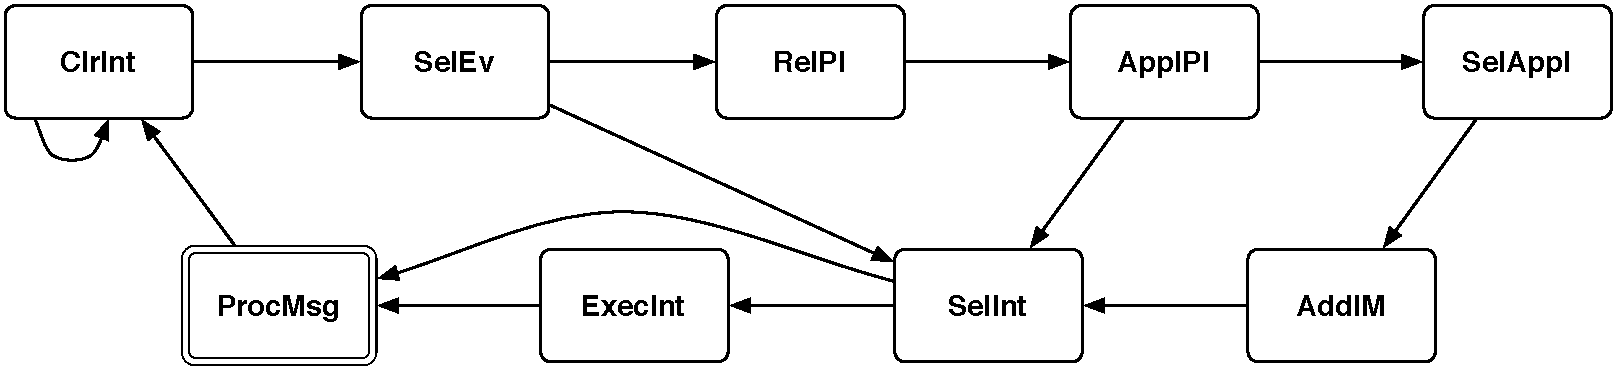
\includegraphics[width=\linewidth]{ASERrc.pdf}
    \caption{The AgentSpeak(ER) Reasoning Cycle}
    \label{fig:rcaser}
  \end{center}
\end{figure}

The $\ClrInt$ stage also needs new semantic rules. In fact, the
previous 3 \rn{ClrInt} rules (see~\cite[p~212]{JasonBook}) are no
longer needed, as empty intentions are not to be removed from the set
of intentions, unless their goal condition becomes true. To facilitate
the presentation of the new rules, we define a new auxiliary function
$\GCOND$, which given a g-plan simply returns the goal-condition
component of that plan, as follows. Let $p=$``\texttt{+!g : c <: gc
  \{<- a.\}}'', then $\GCOND(p)=\texttt{gc}$, more specifically the
logical formula coded by \texttt{gc}. Also, we denote by
$[p_1,...,p_n]$ an intention stack with plan $p_n$ at its top.

The new rule \rn{ClrInt$_1$} is as shown below, and rule
\rn{ClrInt$_1$} is not shown because it simply causes the transition
$\CFG{\ClrInt} \trans \CFG{\SelEv}$ in case the negation of the
precondition of \rn{ClrInt$_1$} holds. The rule below essentially
removes from intentions the bottom-most g-plan for which its
goal-condition now follows from the state of the belief base. The
intuition is that if goal $\texttt{!g1}$ required a subgoal
$\mathtt{!g2}$ (a plan for which was pushed on top of the plan for the
former one in the intention stack) and $\texttt{!g1}$ is no longer
active, that whole part of the intention stack above it needs to be
removed together with it.

\infrule[ClrInt$_1$] {
        i \in \CI \qquad i=[p_1,\dots,p_n] \\
        \AGBELS \models \GCOND(p_j) \mbox{ for some } j, 1\leq j\leq n
}
%------------------------------------------------
{   \CFG{\ClrInt}  \trans  \CFGcp{\ClrInt} \\[1.2mm]  
\begin{array}{llcl}
  \mbox{\emph{where:}\quad}
     & \multicolumn{3}{l}{\mbox{$j$ is the least number in [1..n]
       s.t.}}\\
     & & & \AGBELS \models \GCOND(p_j)\\
     & \CIli & = & \CI \setminus \{i\} \cup \{[p_1,\ldots,p_{j-1}]\} \\
\end{array}
}

The auxiliary functions $\RELPLANS(\PLANS,\TE)$
$\APPLPLANS(\PLANS,\TE)$ (see Definitions~10.2 and~10.3
in~\cite{JasonBook}) can be changed to accommodate both the new g-plan
structure as well as the firing of e-plans (i.e., plans for reacting
to external events) for all intentions rather than creating a single
new separate intention as before. First, the redefined functions now
receive a set of intentions as an extra parameter; in the new semantic
rules they are called with the agent's plan library and the current
contents of the set of intentions ($\AGPLANS$ and$\CI$ in the
operational semantics, respectively). If $\TE$ is an external event,
the new parameter is used to check for applicable plans for each
individual intention plus the empty intention\footnote{The empty
  intention being included in the set of intentions in that parameter
  is useful for backwards compatibility with traditional AgentSpeak(L)
  but we do not discuss this here as it would hinder the explanation
  of the essential aspects of the proposed extension.}
$\EXT$. Besides having an extra parameter, the functions now return a
set of triples rather than a pair. We use $\TREV(p)$ to refer to the
triggering event of a plan $p$, and $\SCOPE([\PL_1,\ldots,\PL_n])$
returns all plans in the scope of the g-plan $p_n$. By ``in scope'',
we mean the plans that appear (immediately) within the braces
delimiting a g-plan (but not within its subgoals); for example the
plans for \texttt{+e1}, \texttt{+e2}, and \texttt{+!k} (but not for
\texttt{+e3}) are in the scope of the g-plan \texttt{+!g : c <: gc \{
  $\ldots$ \}} shown in the beginning of
Section~\ref{sec:infSS}. Furthermore, note that the $\SCOPE$ function
can determine the exact plan for $\PL_n$ in the forest of g-plan trees
now forming the plan library by using plans
$\PL_1,\ldots,\PL_{n-1}$. We can now formally define $\RELPLANS$:

\begin{definition}[Relevant Plans]
  The auxiliary function to retrieve relevant plans given a plan
  library $PL$, a particular event $\TE$ of type \texttt{+l} or
  \texttt{-l} (i.e., an external event, one reacting to changes in
  beliefs rather than a goal adoption event), and a set of intentions
  $I$ is defined as
  $\RELPLANS(PL,\TE,I) = \{ \langle\PLANS,\theta,i\rangle \mid i \in
  I, i = [\PL_1,\ldots,\PL_n],$
  and
  $ps = \{ rp \mid rp \in \SCOPE([\PL_1,\ldots,\PL_j]) \mbox{ and }
  \{\TE\} \models \TREV(rp)\theta$,
  for some m.g.u.\ $\theta\}$, where $j$ is the greatest number in
  $[1..n]$ s.t.\ $ps \neq \emptyset$, or $ps=\emptyset$ if there is no
  such $j\}$. For internal events, the function returns a set
  containing a single element $\langle\PLANS,\theta,i\rangle$ where
  $i$ is the specific intention that generated $\TE$ and $\PLANS$ is
  the set of relevant plans using the same idea of scope as above for
  external events.
\end{definition}

We do not formally define the $\APPLPLANS$ function here due to space,
and given that it is trivially extended in a very similar way as in
Definition~\ref{def:relplans} for $\RELPLANS$.

Finally, we need to change the semantics so that not just one but
\emph{all} relevant e-plans are triggered, that is, one for
each active intention, and within a single intention starting from the
most specific plan (i.e., the one closest to the top of the intention
if there are relevant plans at other levels too). Most of the work was
already done in the redefinitions of the $\RELPLANS$ and $\APPLPLANS$
functions, but we still need to change the rule for processing
external events (which now change multiple intentions). Note however
that by the time we come to handle an external event with rule
\rn{ExtEv}, a single plan for each intention has already been
selected; that is, $\SO$ (the option selection function) is also
slightly redefined to work with the new structures returned by those
redefined auxiliary functions.

The new \rn{ExtEv} rule is below, and it essentially says that an
external event now potentially interrupts various intentions, provided
there are relevant and applicable plans anywhere in the g-plans
associated with each particular current intention of the agent. The
$\TRHO$ component of the transition system configuration has the
result of the application of the new $\RELPLANS$ and $\APPLPLANS$
functions.
% Recall that external events for the ``main'' goal --- the external
% events as in traditional AgentSpeak --- will now be associated with
% the empty intention \EXT in \TRHO (i.e., the result of the
% $\RELPLANS$ and $\APPLPLANS$ functions).
The chosen plan for each intention, after being applied its respective
variable substitution $\theta$, is pushed on top of that intention
(the notation used for this below is $i_j[\PL_j\theta_j]$).

\infrule[ExtEv] {
        \TEPS = \langle\TE,\EXT\rangle \qquad \TRHO =
        \{\langle\PL_1,\theta_1,i_1\rangle,\ldots,\langle\PL_n,\theta_n,i_n\rangle\}
}
%------------------------------------------------
{   \CFG{\ClrInt}  \trans  \CFGcp{\ClrInt} \\[1.2mm]  
\begin{array}{llcl}
  \mbox{\emph{where:}\quad}
     & \CIli & = & \CI \setminus \bigcup_{j=1}^{n} \{i_j\} \cup
                   \bigcup_{j=1}^{n} \{i_j[\PL_j\theta_j] \}\\
\end{array}
}

To conclude this section, we emphasise that, for the sake of space, we
here formalised only the main changes to the well-known AgentSpeak
semantics. The complete new transition system giving semantics to
AgentSpeak(ER) will appear in a longer paper.

\section{Evaluation}
\label{sec:evaluation}
The new language has been evaluated through a prototype implementation that builds on 
the ASTRA \cite{DBLP:conf/prima/CollierRL15} language. This prototype, which is compatible
with pure ASTRA code, is used to reimplement part of an existing solution for the Minority 
Game \cite{moro2004minority}. Interpreter cycle timings are then captured to develop an initial
understanding of how the new language performs.

{\small
\begin{verbatim}
g-plan +!g() : c <: gc { 
  body {
    // main plan body goes here...
    a; b; !g1(); !!g2();
  }

  /* e-plans */
  rule +e1 : c1 { b1; }
  rule +e2 : c2 { b2; }
}
\end{verbatim}}

As can be seen in the  snippet of code above, the implementation of the {\aser} prototype is 
syntactically different to the example provided in section \ref{sec:proposal}. This reflects 
the syntactic approach adopted in ASTRA. It does not impact the associated semantics.

\subsection{Minority Game}
\label{minority}
The Minority Game is a well known model for evaluating collective behaviour of agents competing 
for finite resources \cite{moro2004minority}. In a nutshell, the game involves an odd number of
agents competing for a resource over a series of rounds. For a round, each agent makes a binary
decision (yes/no). At the end of the round, the bids are counted, and the agents that are in the
minority win. The game has been applied mainly in the area of modelling financial markets \cite{??}.

To provide an initial evaluation of {\aser}, we adapt an existing ASTRA-based implementation of 
the Minority Game MG). As is shown in figure \ref{fig:mgagents}, the implementation consists of
3 types of agent: the \emph{compere} agent, who is responsible for managing the game (starting 
rounds, evaluating bids, ...); the \emph{player} agent, who implements a set of MG strategies; 
and the \emph{main} agent, which is responsible for configuring the game (creating and configuring
the compere and player agents). Interaction between the Compere and the Players is through a shared 
game-board artifact.

\begin{figure}[!tbh]
\centering
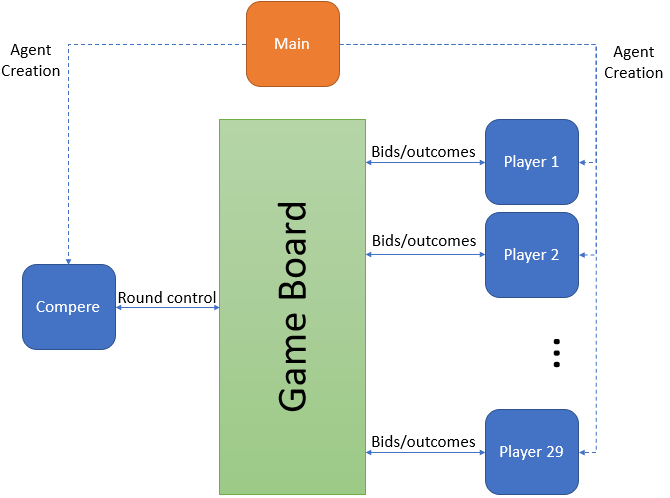
\includegraphics[height=2in, width=2.5in]{mg.png}
\caption{Minority Game Agent Architecture}
\label{fig:mgagents}
\end{figure}

The existing implementation currently consists of 10 plans. Two of the plans are generic and are
used for configuration. Another plan implements the bidding behaviour, delegating to a 
\verb|!select_bid(...)| sub goal that can be contextually selected based on the current strategy.
Of the remaining plans: four relate to the best play strategy; one relates to a random strategy;
and two relate to a sticky strategy.


In the {\aser} implementation, we reduce this to 3 g-plans - one for each of the strategies - 
and one traditional plan to handle initialization. The code below consists of the initialisation 
plan and a single g-plan representating the revised implementation of the best play strategy.

In the code below, the variable A represents the game board, which is implemented as an ASTRA module 
\cite{DBLP:conf/prima/CollierRL15}. Modules allow the developer to create custom actions, 
sensors, (logical) terms, (logical) formulae, and events. For example, \verb|A.join()| is a 
custom action to allow the agent to join the game board; \verb|A.match(history, hist)| is a 
custom term that return the length of the longest common suffix of the \verb|history| and 
\verb|hist| lists; and \verb|$A.event(...)| is a custom event that is generated when the 
Compere agent starts a new round.

The initialisation plan selects the game strategy to be employed by the player. This information
 is passed via the \verb|main(...)| goal; the ASTRA equivalent of a main method. When the handles
the event corresponding to this goal, it spawns a new intention to achieve the \verb|win(...)| 
goal (spawning is like forking in multi-processing and is denoted the double exclamation mark).

In the case that the chosen strategy is \emph{bestplay}, the agent achieves the goal by selecting 
the \verb|!win("bestplay", ...)| g-plan. Upon adoption, the body of this plan is executed, which 
in this case creates a random set of strategies that are to be used by the agent to select its 
bid. This involves adopting the \verb|!setup_tactic()| subgoal which is handled by the first two 
rules within the g-plan. The start of a round is modelled through the custom event 
\verb|$A.event("play", [])|. The rule that is selected to handle this event chooses the best 
strategy from the set of strategies available to the agent. Finally, the end of a round is modelled 
through the custom event \verb|$A.event("winner", [int bid])|. The rule that is selected to handle 
this event updates the score for all strategies that lead to \verb|bid| being selected.

{\small
\begin{verbatim}
rule +!main([string strategy, list config]) {
  !!win(strategy, config); A.join();
}

g-plan +!win("bestplay", [int t, int h]) <: false {
  body { !setup_tactic(t); }

  rule +!setup_tactic(0) {}
  rule +!setup_tactic(int t2) {
    list hist = [];
			
    // construct a random history
    int i=0;
    while (i<h) {
      hist = hist + [M.randomInt() % 2];
      i++;
    }
    +strategy(t2, hist, M.randomInt() % 2);
    +score(t2, 0);
		
    !setup_tactic(t2-1);
  }
		
  rule $A.event("play", []) { 
    list history = A.results();
			
    int max_len = -1; int max_choice = -1;
    int max_score = -1;
    foreach (strategy(int s, list hist, int c) 
              & score(s, int sc)) {
      int len = A.match(history, hist);
      if ((len > max_len) | 
          ((len == max_len) & (max_score < sc))) {
        max_choice = c; max_score = sc;
        max_len = len;
      }
    }
    A.bid(max_choice);
  }

  rule $A.event("winner", [int bid]) {
    foreach (strategy(int s, list hist, bid) 
           & score(s, int sc)) {
      -+score(s, sc+1);
    }
  }
}
\end{verbatim}}

Some interesting observations from adapting the code were: (i) the compexity of the plan contexts 
were simplified when using g-plans because the g-plan itself provided some of the context; (ii) 
the number of arguments passed as parameters was reduced, again because the scope of the parameters 
of the g-plan was the plan body \emph|and| all of its sub-plans; (iii) the total number of rules 
under consideration on each iteration was significantly less because only the rules within an 
active g-plan were considered by the agent - for example, in the original implementation, there 
was always at least one applicable \verb|+!select_bid()| plan per strategy, however in the new 
implementation, only the plans related to the current strategy were applicable.

\subsection{Preliminary Analysis}
\label{performance}

We evaluate the prototype by comparing the {\aser} and ASTRA implementations. Initially,
we compared interpreter cycle execution time and the number of iteration based on a
single configuration of the MG with 29 players and 1000 rounds. For our results, we averaged
the values across all 29 players and repeated the experiment 5 times.

\begin{table}[]
\centering
\caption{Comparing ASTRA and {\aser}}
\label{comparison}
\begin{tabular}{lll}
                      & ASER    & ASTRA  \\
Cycle Time (ms)             & 0.0017  & 0.0036 \\
Cycles                      & 293,772 & 62,880 \\
Elapsed Execution Time (ms) & 495.22  & 229.29 \\
Unix (timed)                & 16s     & 15s   
\end{tabular}
\end{table}

Results of our initial comparison can be found in table \ref{comparison}. The difference
in the number of cycles is due primarily to the scheduling algorithm used by ASTRA, which
suspends agents that have no sensors (perceptors) and whose event and intention queues are empty.
The impact of this is that ASTRA is generally more efficient than {\aser}. Due to the small but 
consistent difference in performance between the unix timing of the two experiments, we then 
explored how increasing the number of rounds affected performance. Results for this are shown 
in table \ref{rounds}.

\begin{table}[]
\centering
\caption{ASTRA vs {\aser} performance}
\label{rounds}
\begin{tabular}{llllll}
           & 1000   & 2000   & 3000   & 4000   & 10000   \\
ASER (s)   & 15.514 & 30.251 & 44.202 & 57.736 & 140.059 \\
ASTRA (s)  & 14.893 & 28.232 & 42.168 & 56.453 & 137.379 \\
Diff. (\%) & 4.2\%  & 6.8\%  & 4.8\%  & 2.3\%  & 2.0\%  
\end{tabular}
\end{table}

This second table shows that {\aser} has a small impact on performance, but it is 
almost linear in this case (ASTRA shows a performance improvement of between 2-6%).

While this is not a thorough evaluation of {\aser}, it does hint that the use of
goal conditions does not significantly impact the performance of the language. It 
must also be noted that the prototype implementation is not as mature as the ASTRA
implementation - interpreter optimisations could further reduce the difference 
in performance.


\section{Related Work}
\label{sec:related}

%% RHB: OK to change this title as below?
%\section{Conclusion and Future Work}
\section{Conclusion}
\label{sec:conclusion}

In this paper, we introduced \aser, a novel extension of the classical
{\asl} language. The language provides encapsulation for agent
goals, which clearly improves legibility and reusability of AgentSpeak
code. Furthermore, the new language improves some of the shortcomings
of AgentSpeak in regards to goal orientation and declarative goals by
ensuring that all reactive plans are also associated with general
goals, providing a ``goal condition'' which means goals can be still
active even though presently there is no action for the agent to take
towards that goal, and allowing external events (i.e., reactions to
changes in beliefs) to trigger various plans, for all the goals it
might be relevant.  We formalised the main changes required in the
existing formal semantics of AgentSpeak and experimentally evaluated
an interpreter for \aser\ implemented on top of the ASTRA platform.

As with any new programming language, there is much future work, some
in fact ongoing. We are currently refining the ASTRA implementation,
trying to make a few optimisations to improve the evaluation results we
reported in this paper. A Jason-based implementation is also under
way; comparison of the performances of the two implementations might
lead to insight that might improve the implementation of the platforms
themselves. 

More generally, full understanding and evaluation of a programming
language takes many years. We expect in the long term to use \aser\ in
the practical development of multi-agent systems, both for real-world
systems and also academic ones (e.g., for the multi-agent
programming contest~\cite{??}). However, besides the actual
programming practice, we expect \aser\ to contribute to formal work as
well. Assessing how formal verification of \aser\ systems compares to
the original language is also planned as future work.
%% RHB: Do we need to cite, perhaps the intro paper of the special
%% issue of the competition for the last year?

% \begin{itemize}
% \item refining current ASTRA implementation, that will allow to refine the evaluation
% \item Jason extension implementing {\aser}, and compare it with the ASTRA one
% \item stress {\aser} in practice 
% \item think about the tools: how existing IDE and tools can be extended to provide functionalities exploiting the new features
% \item investigate how the extension either improve or not the possibility to formally analyse the correctness properties
% \item ...
% \end{itemize}




%%%%%%%%%%%%%%%%%%%%%%%%%%%%%%%%%%%%%%%%%%%%%%%%%%%%%%%%%%%%%%%%%%%%%%%%%%%%%%%%%%%%%%%%%%%%%%%%%%%%%%%%%
%% bibliography: see CFP for number of permitted pages

\bibliographystyle{ACM-Reference-Format}  % do not change this line!
\bibliography{main}  % put name of your .bib file here

\end{document}
